%%%%%%%%%%%%%%%%%%%%%%%%%%%%%%%%%%%%%%%%%
\documentclass[
	12pt, % Default font size, values between 10pt-12pt are allowed
	%letterpaper, % Uncomment for US letter paper size
	%spanish, % Uncomment for Spanish
]{fphw}

% Template-specific packages
\usepackage[utf8]{inputenc} % Required for inputting international characters
\usepackage[T1]{fontenc} % Output font encoding for international characters
\usepackage{mathpazo} % Use the Palatino font
\usepackage{amssymb}
\usepackage{graphicx} % Required for including images

\usepackage{booktabs} % Required for better horizontal rules in tables

\usepackage{listings} % Required for insertion of code

\usepackage{enumerate} % To modify the enumerate environment
\usepackage[super]{nth}
% ----------------------------------------------------------------------------------------

%	ASSIGNMENT INFORMATION
%----------------------------------------------------------------------------------------
 \usepackage{geometry}
 \geometry{
  a4paper,
  total={170mm,257mm},
  left=20mm,
  top=20mm,
  }

\title{IA LAB: Ladder Logic Programmes} % Assignment title
\author{Darsh Gajjar} % Student name
\date{04/01/2021}
\institute{SVNIT, SURAT \\ M. Tech. I \& C (Electrical Department)} % Institute or school name

\class{Industrial Automation LAB} % Course or class name

\professor{Dr. H. G. Patel} % Professor or teacher in charge of the assignment

%----------------------------------------------------------------------------------------

\begin{document}
\maketitle % Output the assignment title, created automatically using the information in the custom commands above
%----------------------------------------------------------------------------------------
%	ASSIGNMENT CONTENT
%----------------------------------------------------------------------------------------
\pagebreak

\section*{Program \#1}

\begin{problem}
  There is Big godown in which there are 3 sensors installed,
  \medskip
  \begin{itemize} 
   \item If any one sensor is on then indicators ON,
   \item If any two sensors on then hooters ON,
   \item If all sensors are ON then Fire extinguisher should be ON
  \end{itemize}
\end{problem}
%------------------------------------------------
\subsection*{Answer}
 \begin{center}
 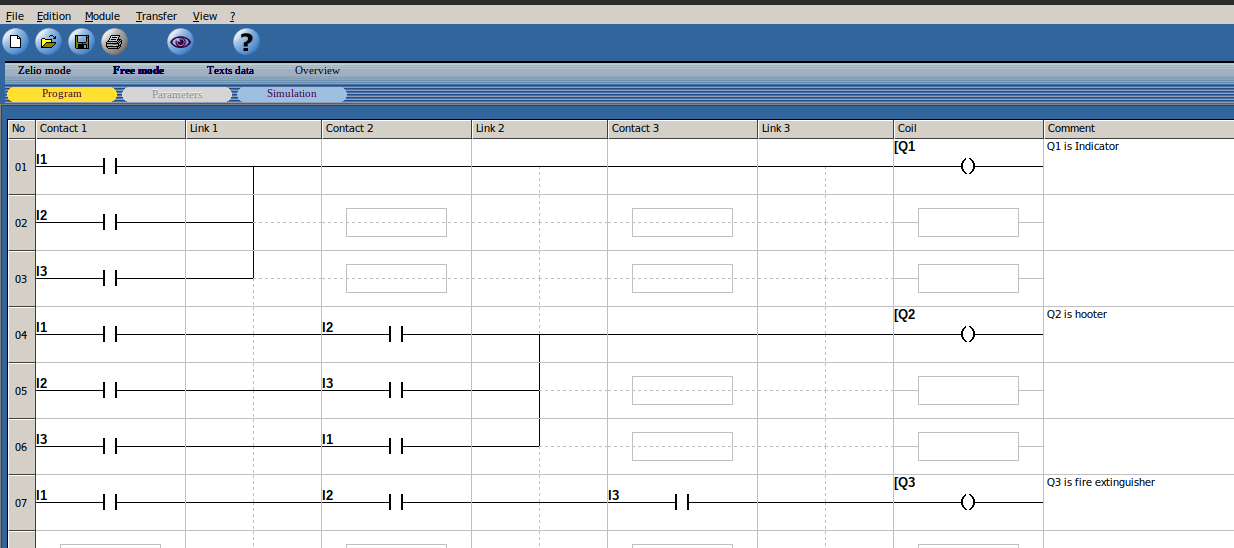
\includegraphics[width=165mm, scale=0.80]{prg1.png} % Example image
\end{center}
% ----------------------------------------------------------------------------------------
\section*{Program \#2}
\begin{problem}
One cutting machine with left and right start switches
\medskip
 \begin{itemize}%[(\itshape a\normalfont)]
  \item If both switches on then machine on
  \item When you release any switch machine off
  \end{itemize}
\end{problem}
\subsection*{Answer}
 \begin{center}
  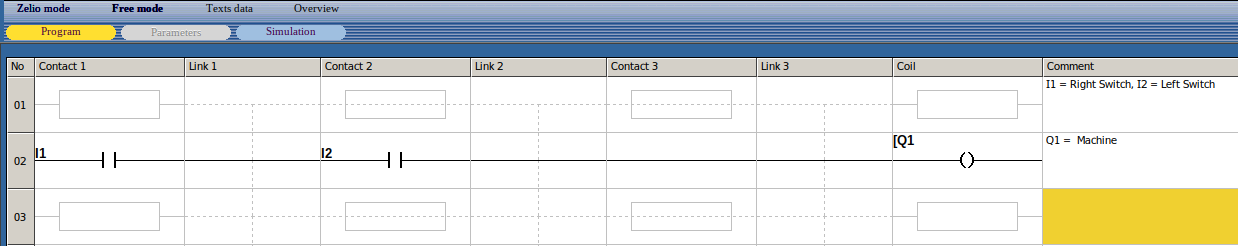
\includegraphics[width=165mm, scale=0.80]{prg2.png}
 \end{center}
  % -------------------------------------------------------------------------------------------------------
\section*{Program \#3}

 \begin{problem}
  whenever we press ON Push button then Motor should remain ON and when STOP
 push button is press it shoulf OFF immediately
 \end{problem}

\subsection*{Answer}
 \begin{center}
  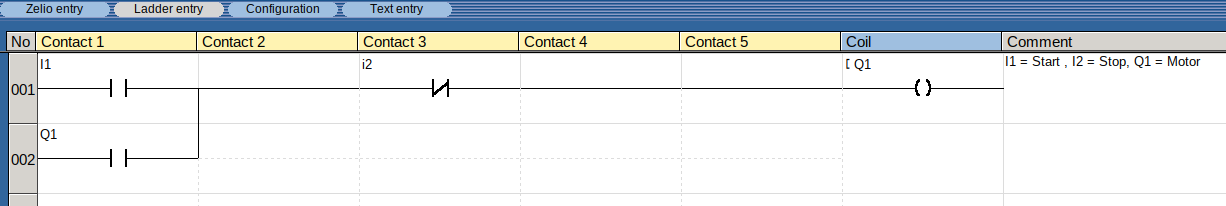
\includegraphics[width=165mm, scale=0.80]{prg3.png}
 \end{center}
  % -----------------------------------------------------------------------------------------------------------------------
\section*{Program \#4}
 \begin{problem}
  In 35 feet long machine design ladder logic by which operator should able to
  Start and Stop from three different place 
 \end{problem}

\subsection*{Answer}
 \begin{center}
 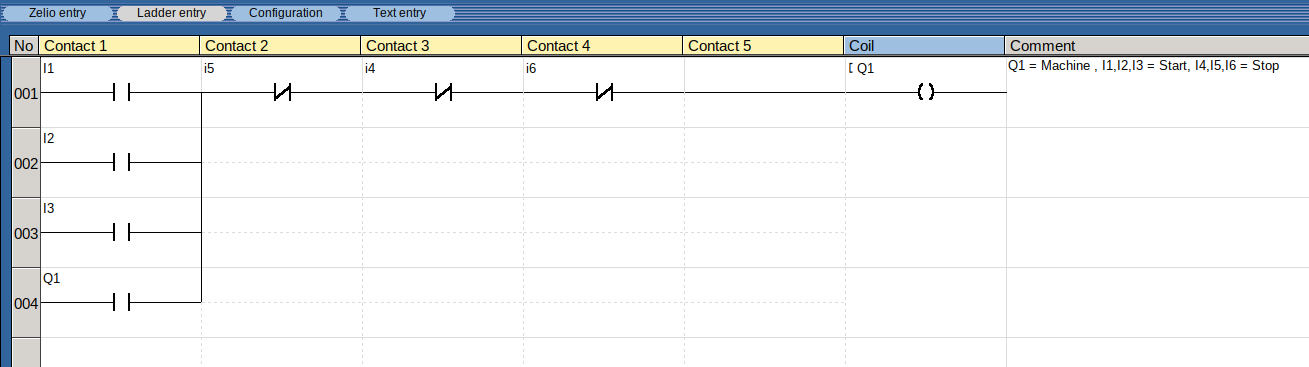
\includegraphics[width=165mm, scale=0.80]{prg4.png}
 \end{center}
% ---------------------------------------------------------------------------------------------------------------
\section*{Program \#5}
 \begin{problem}
   There is one lubrication Pump and one Motor
 \medskip
 \begin{itemize}%[(\itshape a\normalfont)]
  \item first lubrication Pump should be On and then Motor ON
  \item When STOP Push button is pressed Motor and Pump should be Stop together
  \end{itemize}
\end{problem}
\subsection*{Answer}
\begin{center}
  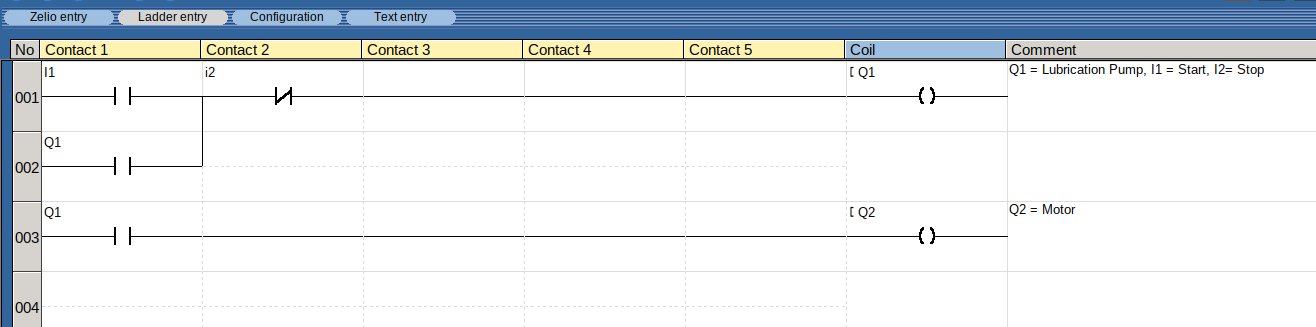
\includegraphics[width=165mm, scale=0.80]{prg5.png}
\end{center}

%% -------------------------------------------------------------------------------------------------------
\section*{Program \#6}                                                           
\begin{problem}                                                           One
  3-phase Induction Motor need to operate in forward/reverse direction when
  motor start operate in forward direction reverse direction should off first
  and when operate in reverse direction then forward direction should off first                                
  \medskip
\end{problem}
\subsection*{Answer}
 \begin{center}
   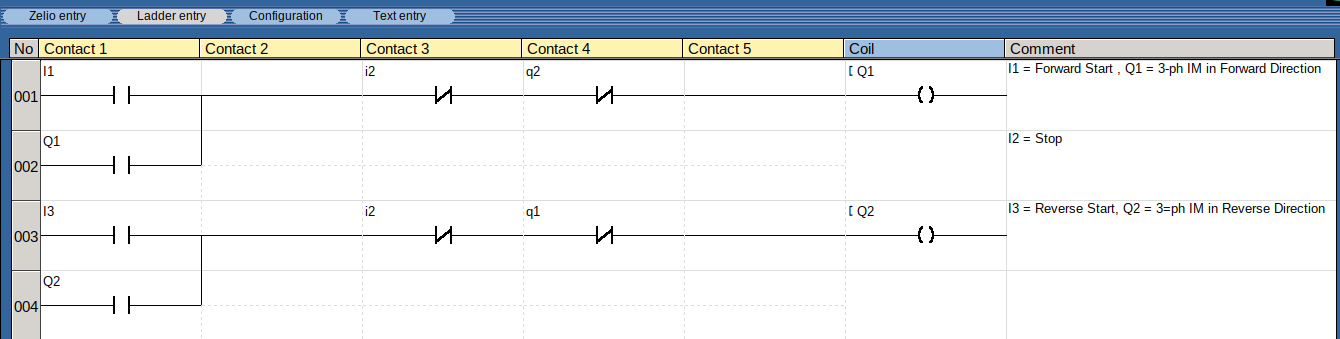
\includegraphics[width=165mm, scale=0.80]{prg6.png}
 \end{center}


\section*{Program \#7}                                                           
\begin{problem}
There is one motor and one pump,when start push buttion is pressed first pump
and afterward motor should start and STOP button is individual.
\medskip
\end{problem}
\subsection*{Answer}
 \begin{center}
  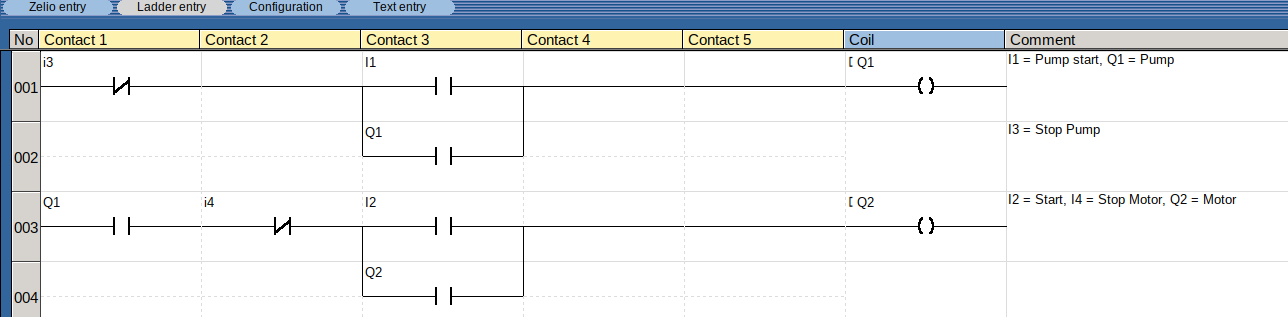
\includegraphics[width=165mm, scale=0.80]{prg7.png}
 \end{center}


\section*{Program \#8}
\begin{problem}
  There are two Motors, in which one should work at one time and other remains
  in standby
  \begin{enumerate}
  \item with Stop Push button
  \item with Set/reset coils
    \item without any STOP push button
  \end{enumerate}
 \medskip
 \end{problem}
 \subsection*{Answer}
 \begin{enumerate}
   \item
  \begin{center}
   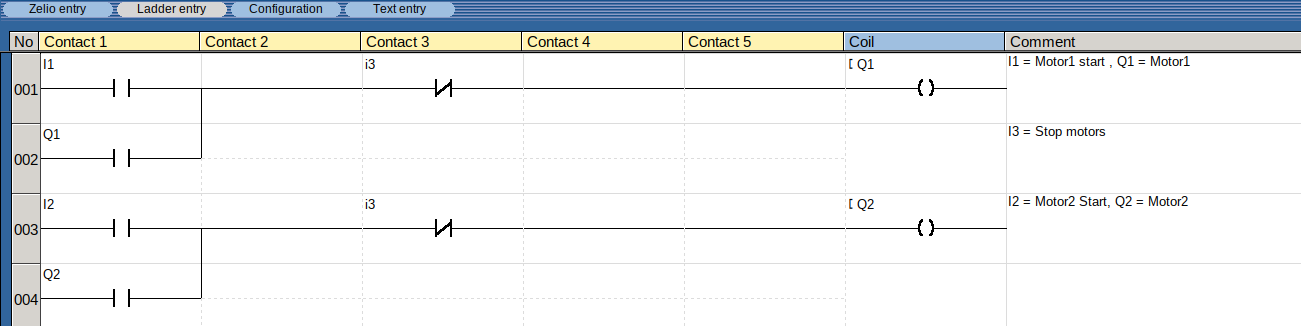
\includegraphics[width=150mm, scale=0.80]{prg8.png}
  \end{center}
   \item
   \begin{center}
    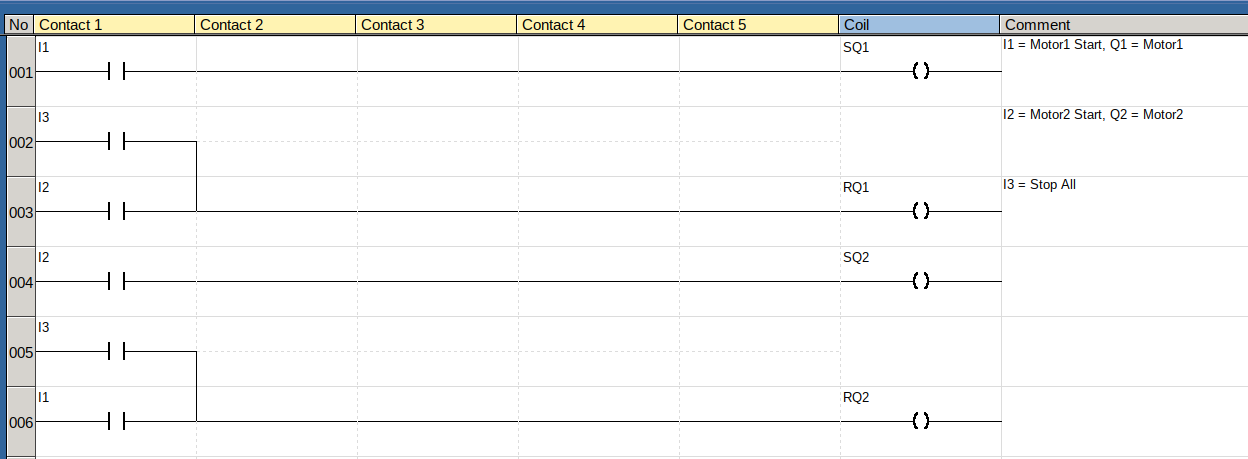
\includegraphics[width=150mm, scale=0.80]{prg9.png}
   \end{center}
  \item
    \begin{center}
     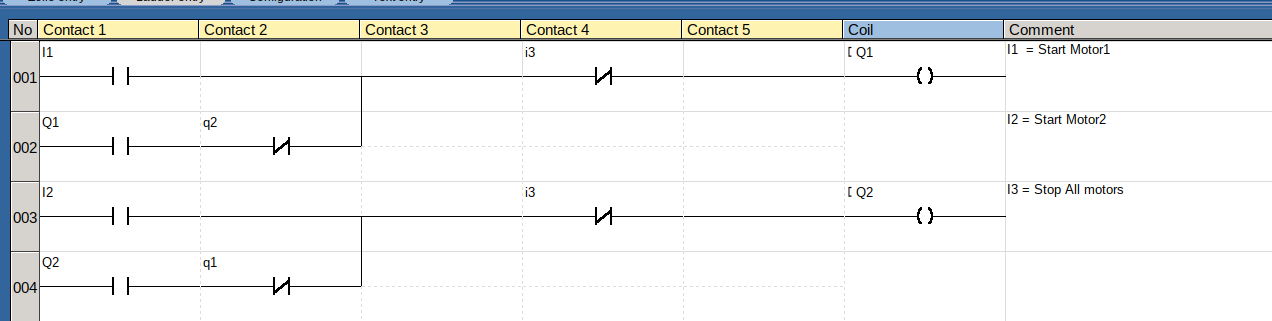
\includegraphics[width=150mm, scale=0.80]{prg10.png}
   \end{center}
 \end{enumerate}
 
%%--------------------------------------------------------------------------------------------------------------------
\section*{Program \#09}
    \begin{problem}
      There are two motors
      \medskip
      \begin{itemize}
      \item start motor1, after 10 second motor2 start automatically
      \item when motor1 stops second one stops automatically
      \end{itemize}
    \end{problem}
\subsection*{Answer}
     \begin{center}
      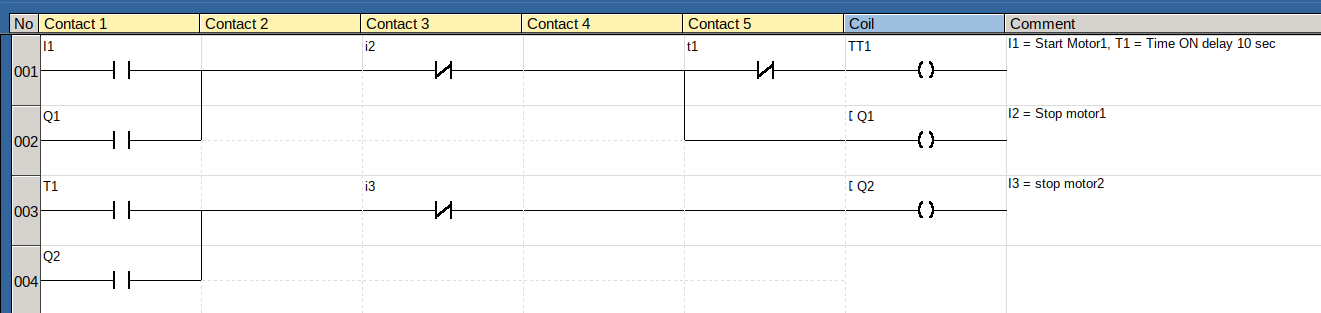
\includegraphics[width=165mm, scale=0.80]{prg11.png}
    \end{center}

\section*{Program \#10}
\begin{problem}
  There are three motors
  \medskip
  \begin{itemize}
  \item when start push button is pressed Motor1 ON
  \item after 5 sec Motor2 ON
  \item after 5 sec Motor3 ON
  \item when STOP push button is pressed all should STOP together
  \end{itemize}
\end{problem}
\subsection*{Answer}
\begin{center}
  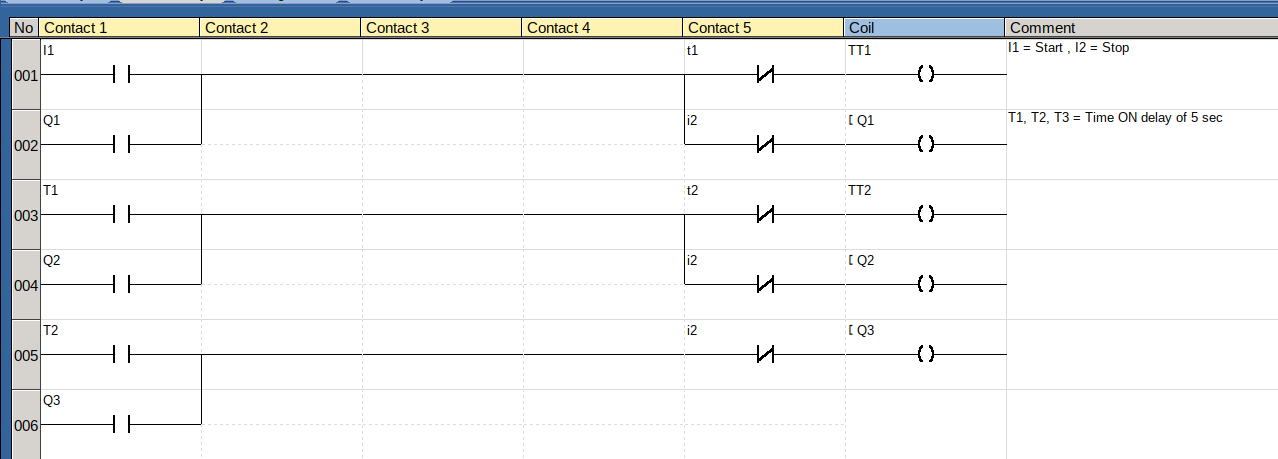
\includegraphics[width=165mm, scale=0.80]{prg12.png}
\end{center}

\section*{Program \#11}
\begin{problem}
  There are two motors
  \medskip
  \begin{itemize}
   \item when start push button is pressed Motor1 ON and then after 5 second
     Motor2 ON
   \item when stop push button is pressed Motor1 off and then after 5 second Motor2 Off
  \end{itemize}
\end{problem}
\subsection*{Answer}
\begin{center}
  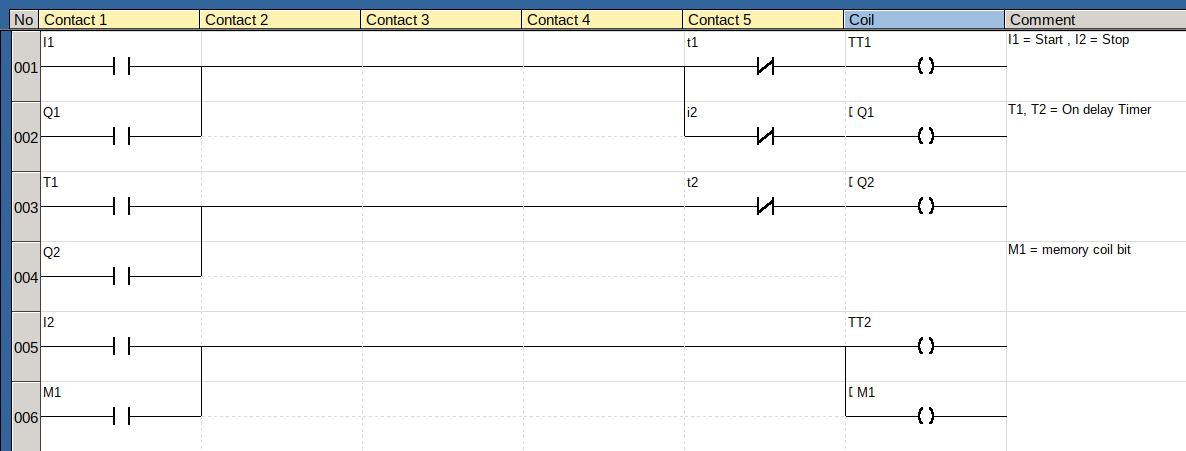
\includegraphics[width=165mm, scale=0.80]{prg13.png}
\end{center}


\section*{Program \#12}
 \begin{problem}
  Consider one wood cutting machine and one blower as soon as wood cutting
  machine starts, blower should start, when wood cutting machine stops, blower
  stop after 10 second
   \medskip
 \end{problem}
\subsection*{Answer}
 \begin{center}
  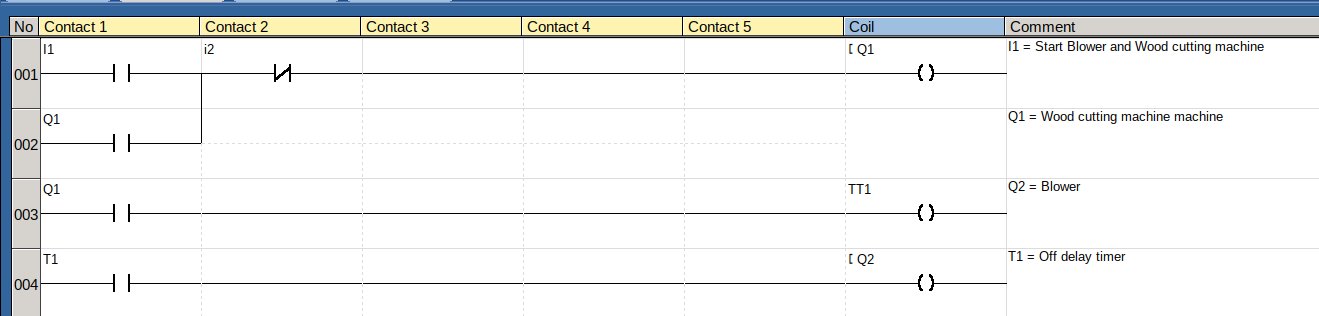
\includegraphics[width=165mm, scale=0.80]{prg14.png}
 \end{center}


\section*{Program \#13}                                                                    
  \begin{problem}
    There are two motors
    \medskip
   \begin{itemize}
    \item Motor1 start immediately after Push button is pressed
    \item After 5 second Motor2 start and Motor1 Stop
    \item After 5 second Motor1 Start and Motor2 Stop
    \end{itemize}
    operate motors alternate mode continuosly
    \begin{enumerate}
    \item Do above logic using set/reset coil bit and two timers
    \item Do above logic using set/reset coil bit and one timer
    \item Do above logic using without set/reset and two timers
    \item Do above logic using without set/reset and One timer
      \end{enumerate}
  \end{problem}
 \subsection*{Answer}
  \begin{enumerate}
   \item using set/reset and two timer  
     \begin{center}
       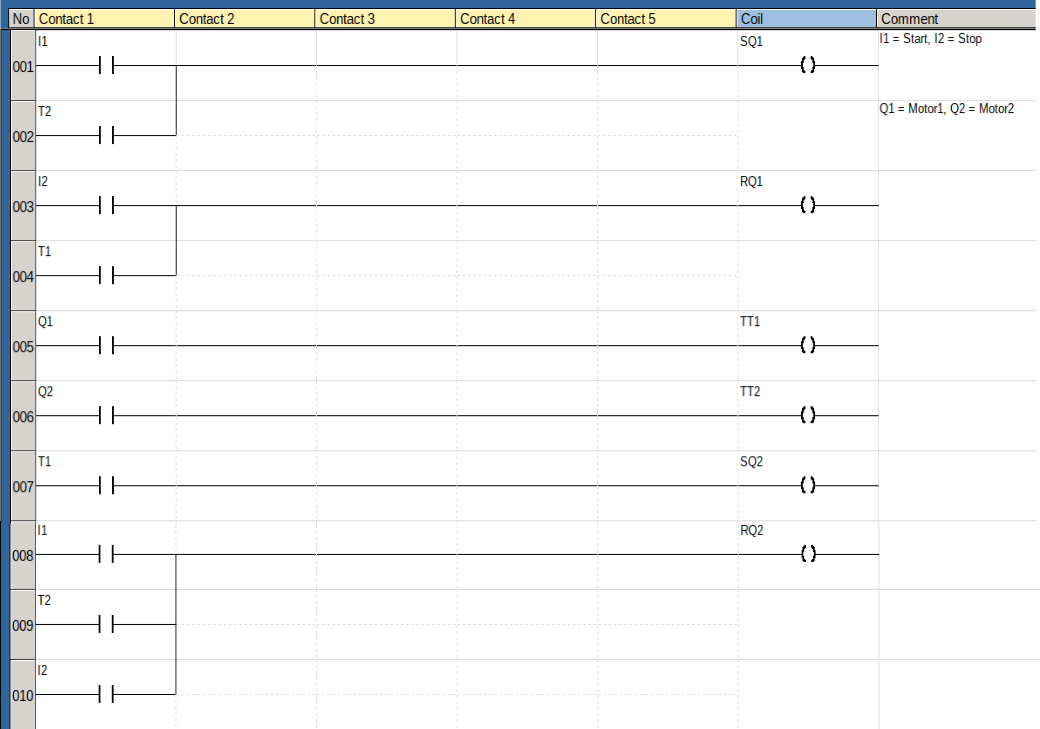
\includegraphics[width=150mm, scale=0.80]{prg15.png}
     \end{center}
   \item using set/reset and one timer
 \begin{center}
   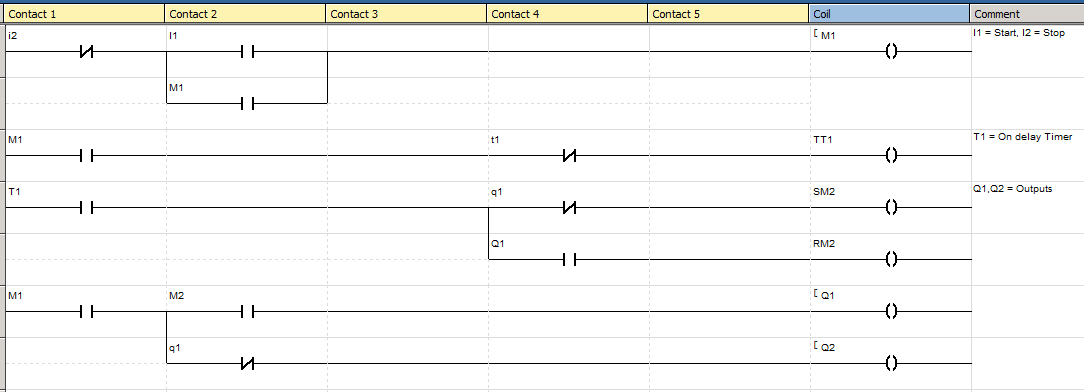
\includegraphics[width=150mm, scale=0.80]{p13b.png}
 \end{center}
   \item without set/reset and two timers
     \begin{center}
       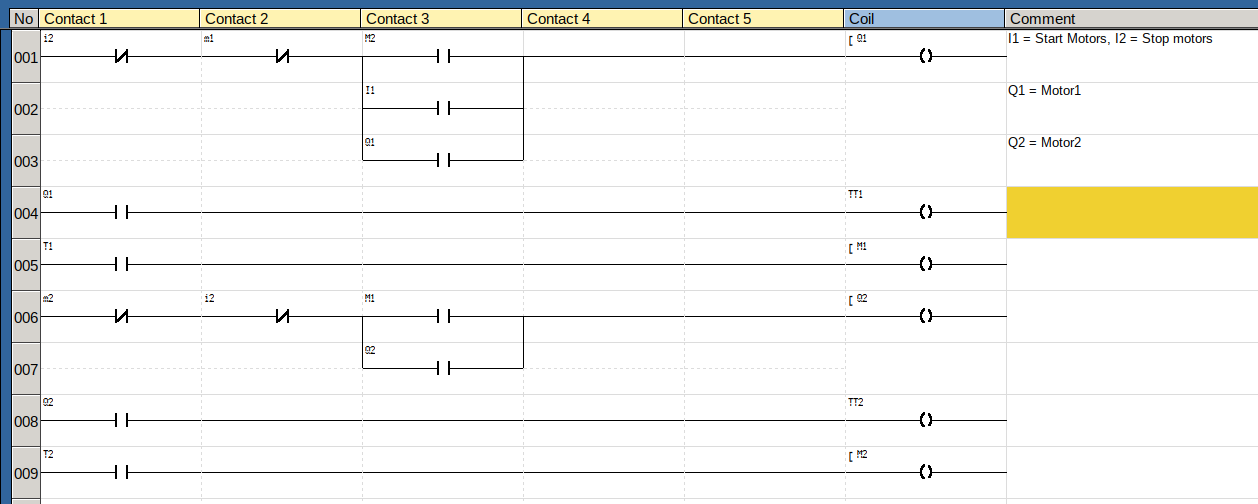
\includegraphics[width=150mm, scale=0.80]{prg16.png}
     \end{center}
   \item without set/reset and one timer
     \begin{center}
       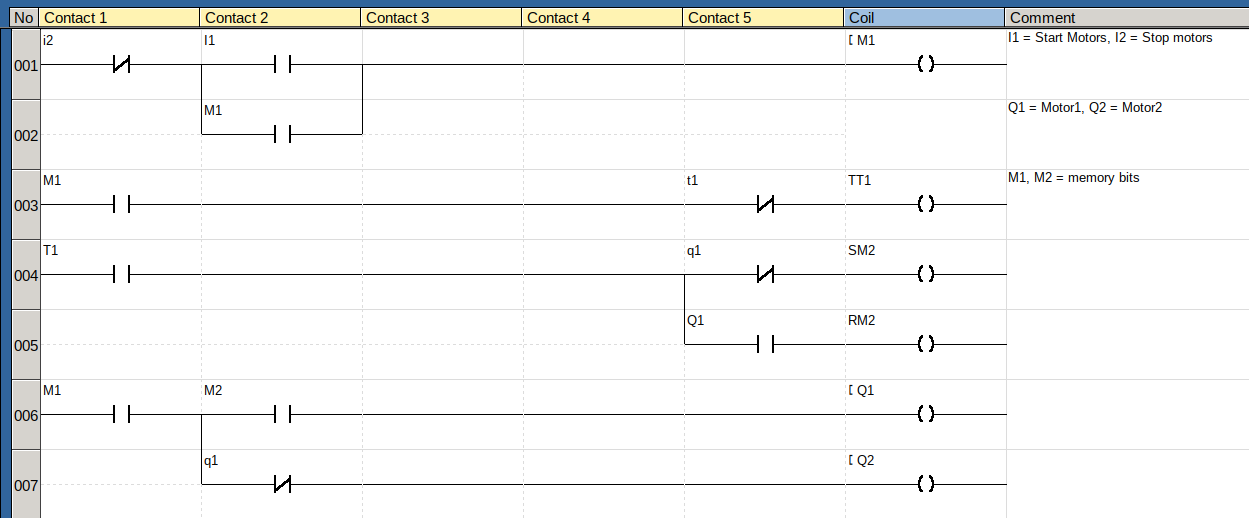
\includegraphics[width=150mm, scale=0.80]{prg17.png}
     \end{center}
    \end{enumerate}
\section*{Program \#14}
 \begin{problem}
   One motor is operate using single push button and then when button pressed
   first motor should be ON and when pressed same button again it should OFF,
   then again if button pressed it should start again.
  \medskip
 \end{problem}
\subsection*{Answer}
  \begin{center}
   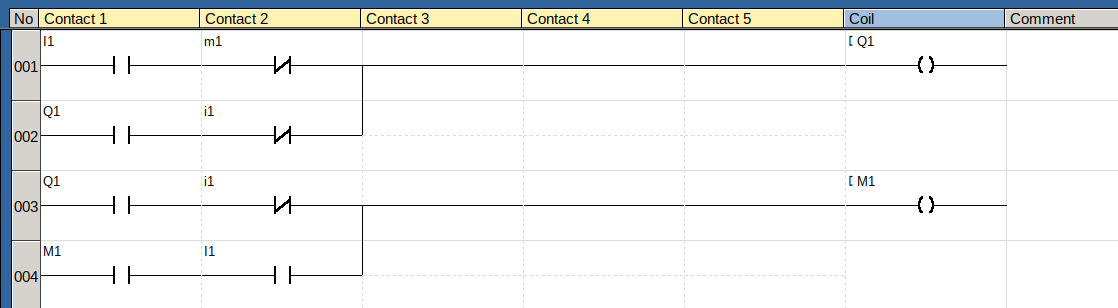
\includegraphics[width=165mm, scale=0.80]{prg18.png}
  \end{center}


 \section*{Program \#15}
  \begin{problem}
    In One bottle filling plant,there are 6 bottles in each box
    \begin{enumerate}
      \item when six bottles are filled \nth{1} indicator should be ON
      \item when 5 such box are packed \nth{2} indicator should be ON
    \end{enumerate}
    \medskip
  \end{problem}
  
 \subsection*{Answer}
 \begin{enumerate}
   \item answer of \nth{1} part
   \begin{center}
   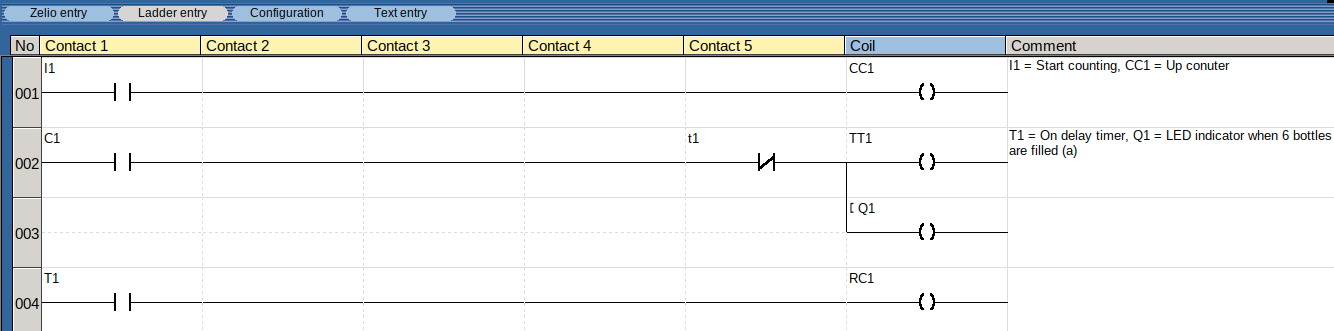
\includegraphics[width=150mm, scale=0.90]{prg17a.png}
   \end{center}
   \item answer of \nth{2} part
   \begin{center}
   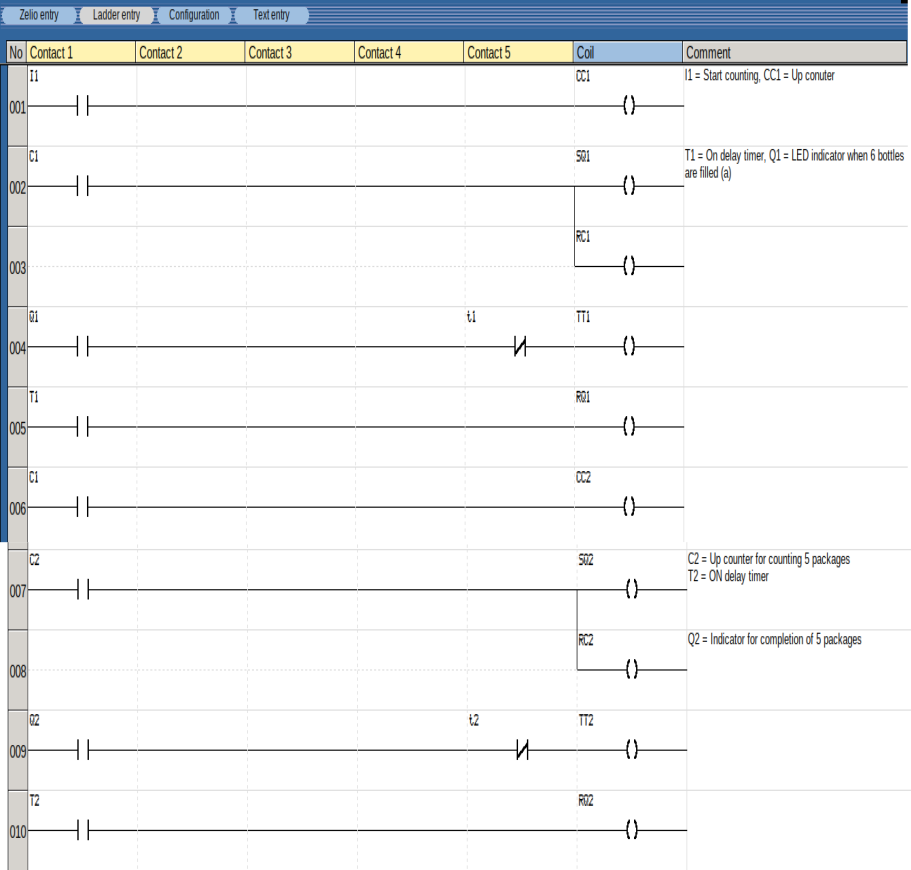
\includegraphics[width=150mm, scale=0.90]{prg20.png}
   \end{center}
  \end{enumerate}

 \section*{Program \#16}
 \begin{problem}
  In Automatic blending process there are sequence of operations are going to
  held as per flowchart and design ladder logic for it. \par
  \medskip
  Flow chart of problem 16
  \begin{center}
    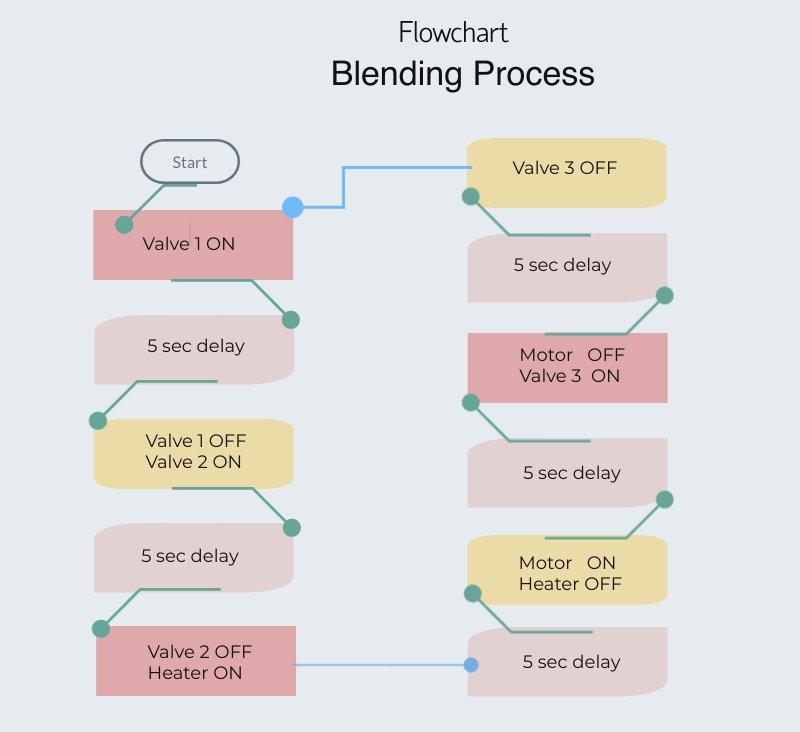
\includegraphics[width = 150mm, scale=0.90]{blending1.jpg}
  \end{center}
  \end{problem}
 \subsection*{Answer}
   \begin{center}
    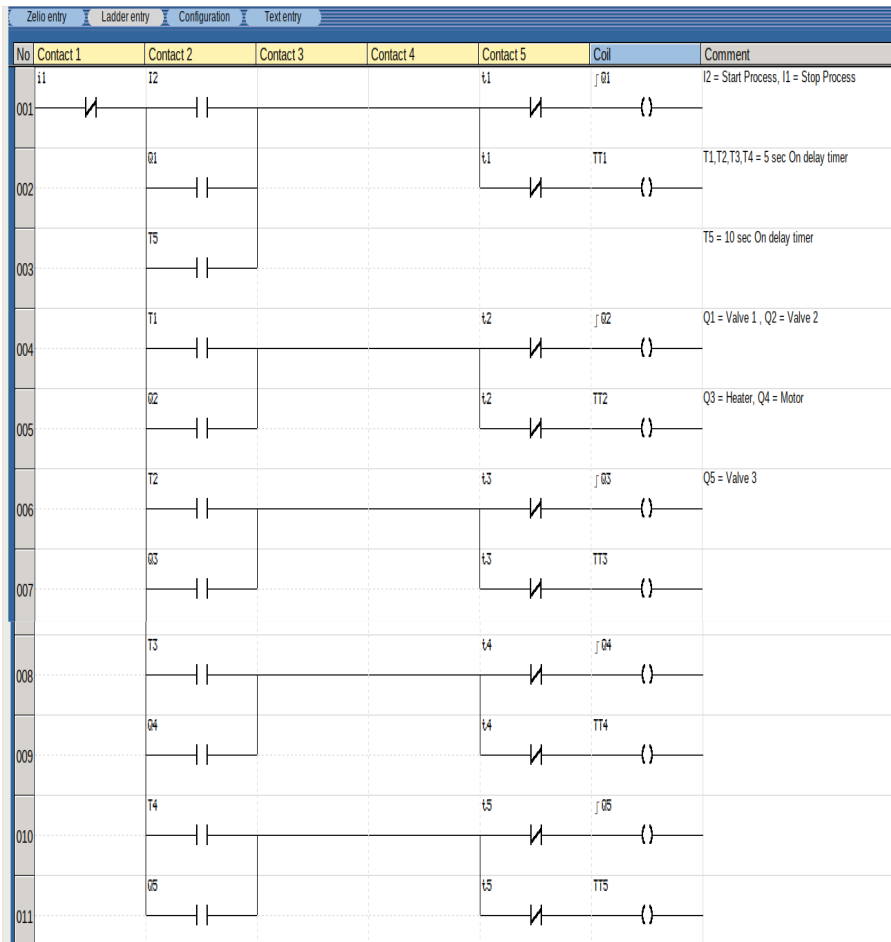
\includegraphics[width= 165mm, scale=0.90]{blender.png}
   \end{center}                                                                


  \section*{Program \#17}
  \begin{problem}
    When Process start One Light blinking at varying frequency as stated below
\medskip
    \begin{itemize}
      \item when \nth{1} push button is pressed Light is On and OFF at every 1
        second
      \item when \nth{2} push button is pressed Light is On and OFF at every 2
        second
      \item when \nth{3} push button is pressed Light is On and OFF at every 3
        second
      \item when \nth{4} push button is pressed Light is flickering at 0.5 Hz
        frequency.
    \end{itemize}
   \end{problem}
  \subsection*{Answer}
  \begin{center}
   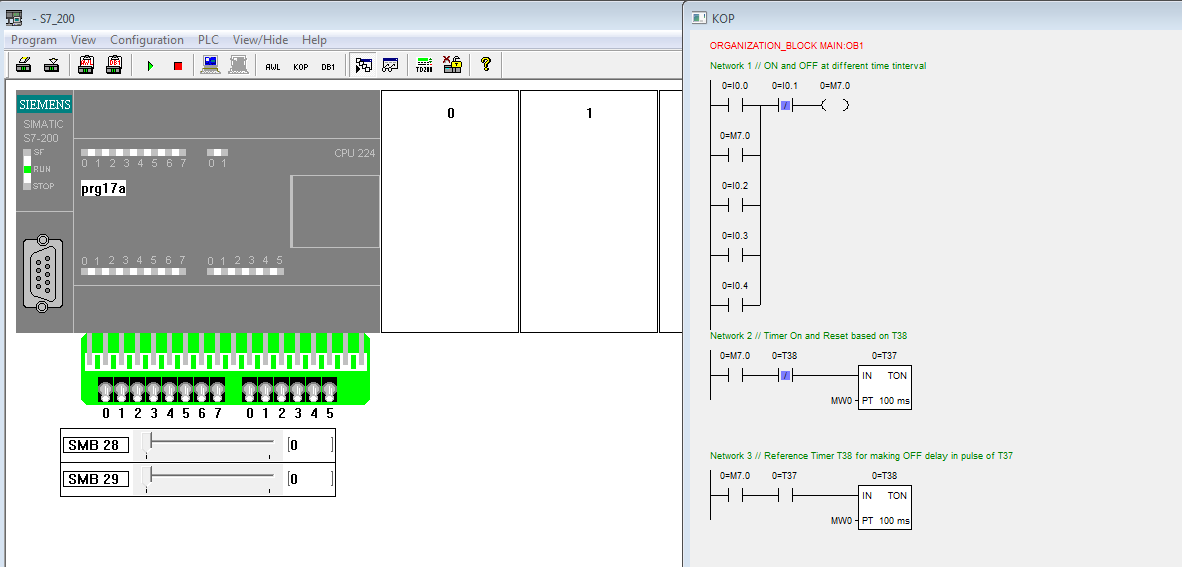
\includegraphics[width=165mm, scale=0.90]{p17a1.png}
   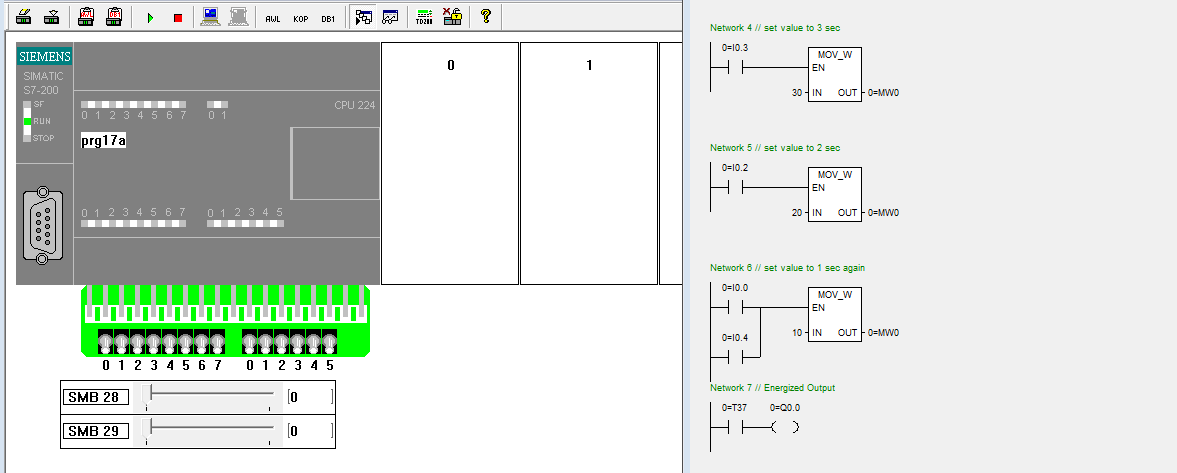
\includegraphics[width=165mm, scale=0.90]{p17a2.png}
 \end{center}

 \section*{Program \#18}
 \begin{problem}
  In one process when start PB is pressed Timer starts  \medskip
 \begin{itemize}
\item when Timer reach to 3 sec PUMP ON
\item when Timer reach to 6 sec Motor ON
\item when Timer reach to 7 sec Motor OFF
\item when Timer reach to 8 sec PUMP OFF
 \end{itemize}
\end{problem}
\subsection*{Answer}
\begin{center}
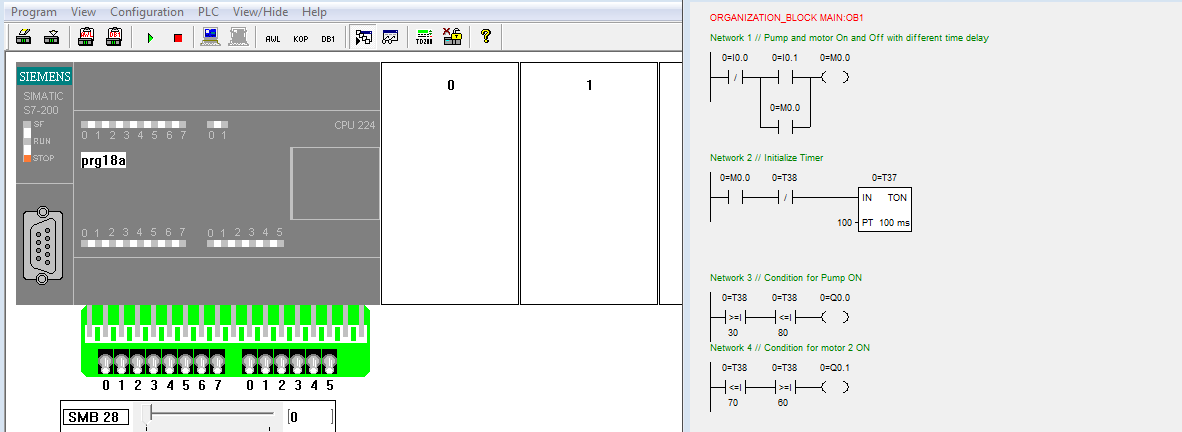
\includegraphics[width=165mm, scale =0.9]{p18a1.png}
\end{center}
\section*{Program \#19}
\begin{problem}
 There are two no of motors, when Start PB is pressed Timer starts \medskip
\begin{itemize}
\item from time interval 0 to 10 sec Motor1 ON
\item from time interval 10 to 20 sec Motor2 ON
\item from time interval 20 to 30 sec Motor1 and Motor2 ON
\end{itemize}
\end{problem}
\subsection*{Answer}
\begin{center}
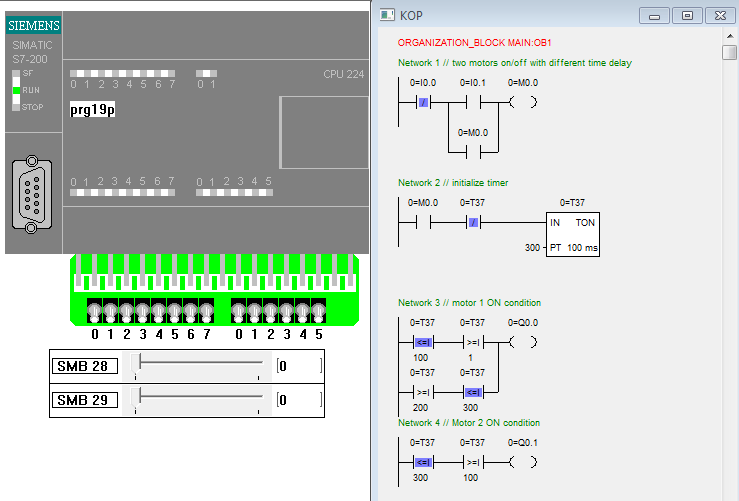
\includegraphics[width = 165mm, scale =0.9]{prg19p.png}
\end{center}
\section*{Program \#20}
\begin{problem}
  There are three no of motors, when Start PB is pressed Timer starts \medskip
\begin{itemize}
 \item from time interval 0 to 10 sec Motor1 \& Motor3 ON
 \item from time interval 10 to 20 sec Motor2 ON
 \item from time interval 20 t0 30 sec Motor2 \& Motor3 ON
 \item from time interval 30 to 40 sec All Motors ON
 \item when time in seconds > 40 sec All motors OFF
\end{itemize}
\end{problem}
\subsection*{Answer}
 \begin{center}
 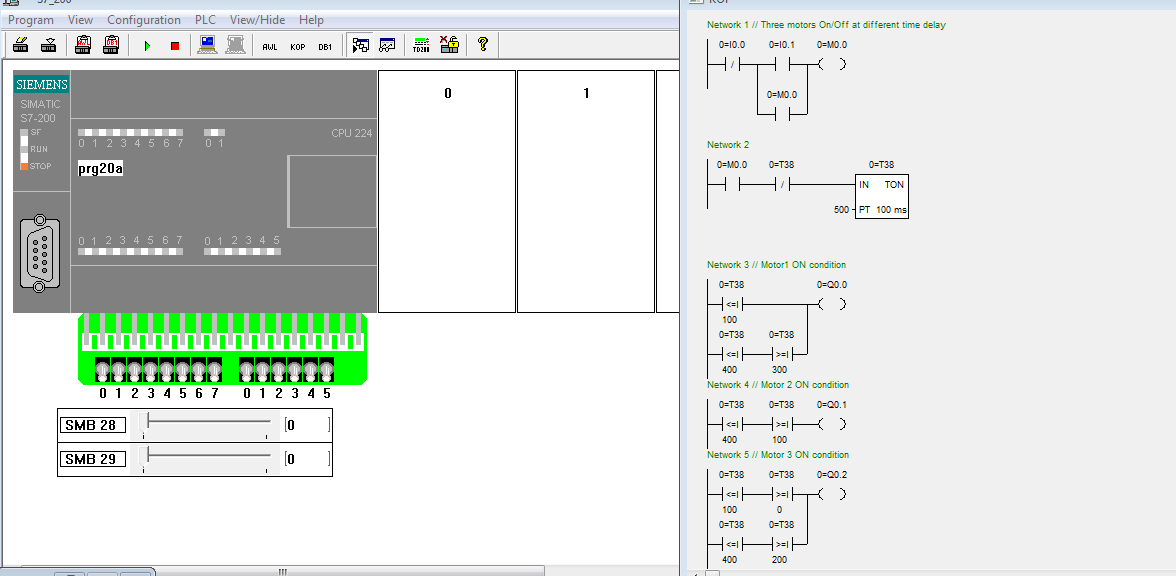
\includegraphics[width = 165mm, scale =0.9]{p20a1.png}
 \end{center}
\section*{Program \#21}
\begin{problem}
  Convert data that stored in Byte into real data Or convert data into \%VBXX
  into Real value.
  \medskip
\end{problem}
\subsection*{Answer}
 \begin{center}
 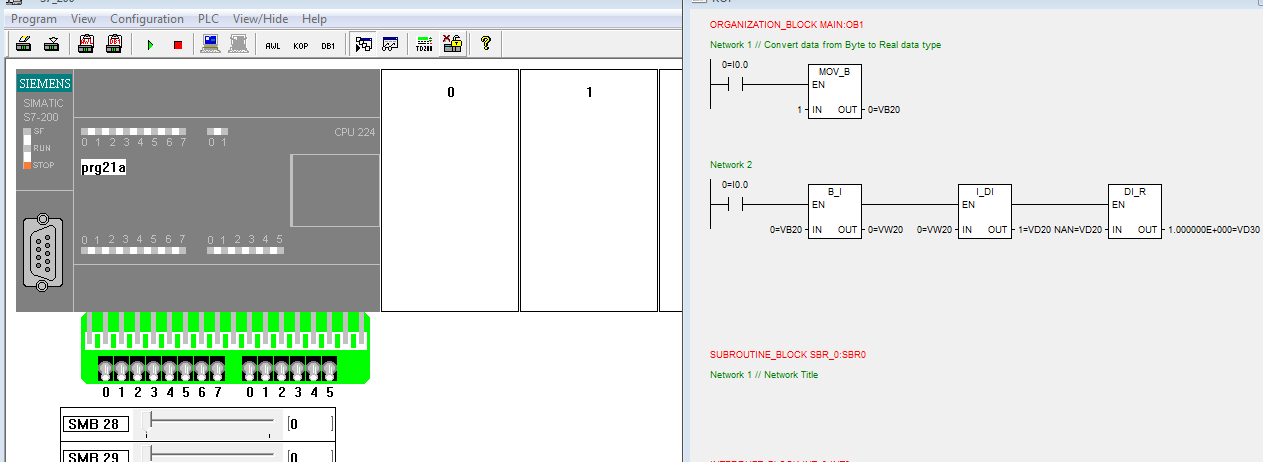
\includegraphics[width = 165mm, scale =0.9]{p21a1.png}
 \end{center}

\section*{Program \#22}
\begin{problem}
  Design a programme in which there is input of data available from User/HMI \medskip
 \begin{itemize}
  \item if input data is $\leq$ 255 then convert it into byte data type and store
    into(\%VBXX) and also energized one output. 
  \item if input data is $\leq$ 32000 and $\geq$ 256 then convert it into integer data type and store
  into(\%VWXX) and also energized two outputs.
\item if input data is $>$ 32000, then energized three outputs.
\end{itemize}
\end{problem}
\subsection*{Answer}
  \begin{center}
    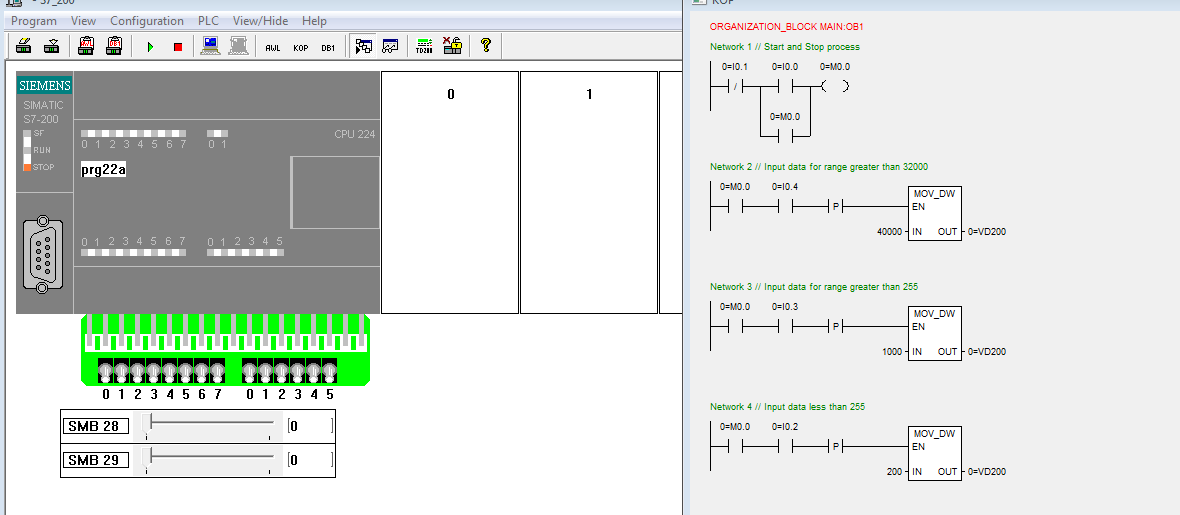
\includegraphics[width = 165mm, scale =0.9]{p22a1.png}
    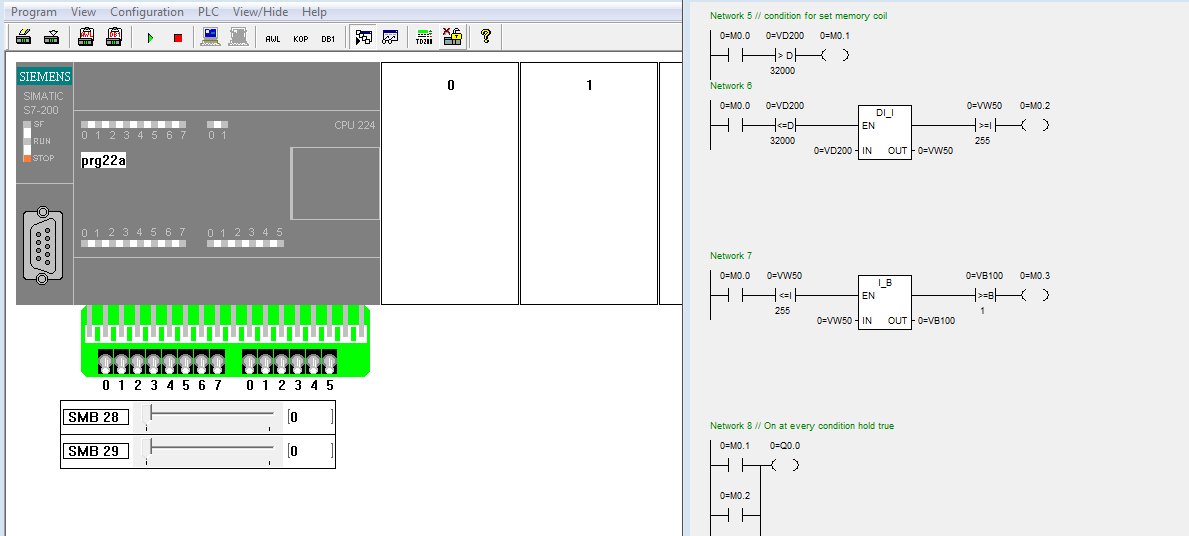
\includegraphics[width = 165mm, scale =0.9]{p22a2.png}
    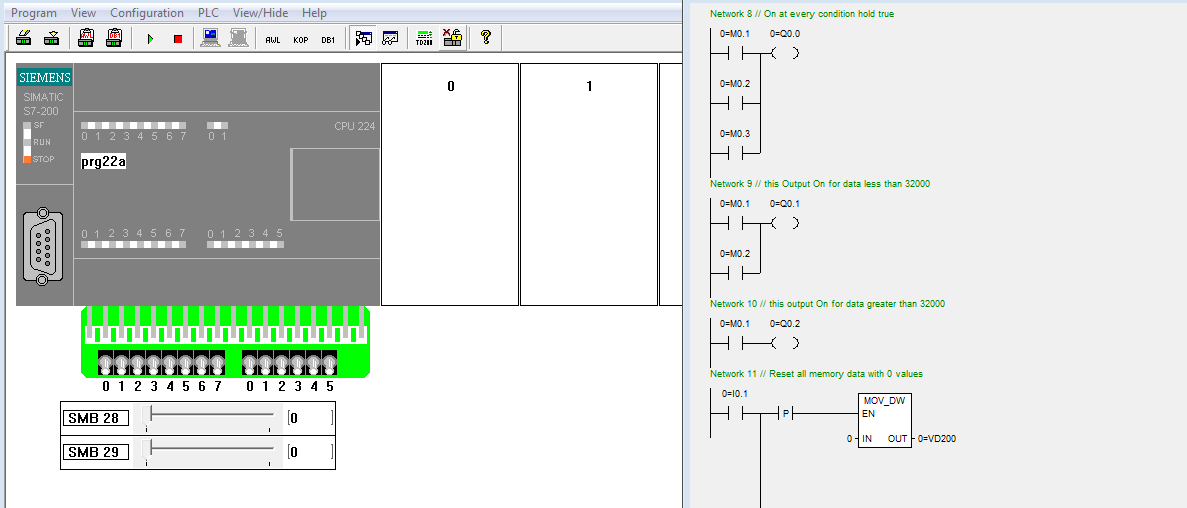
\includegraphics[width = 165mm, scale =0.9]{p22a3.png}
     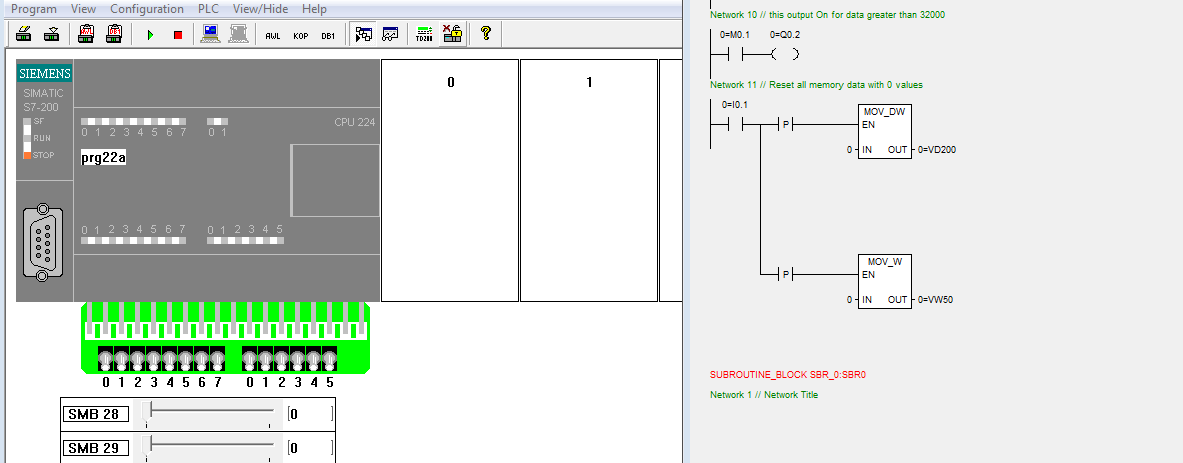
\includegraphics[width = 165mm, scale =0.9]{p22a4.png}
  \end{center}
\section*{Program \#23}
\begin{problem}
 When one Process starts: 1 light On and Off at one seconds(Current time interval = 2(1 sec ON + 1 sec OFF) sec) \medskip
\begin{itemize}
\item when PB1 is pressed same light On and Off at 3 seconds (current time interval + 2) sec
\item When PB2 is pressed same light On and OFF at (current time interval – 2) sec
\item When PB3 is pressed same light On and OFF at (current time interval * 4) sec
\item When PB4 is pressed same Light On and OFF at (current time interval / 4) sec
\item minimum time for On and OFF is 1 second, if above mathematical Operation
  achieves Higher than frequency 0.5 Hz than set it to again at 0.5 Hz.
\item if same button is pressed again particular arithmatic operation as per
  above condition is applied on current time interval
\end{itemize}
\end{problem}
\subsection*{Answer}
\begin{center}
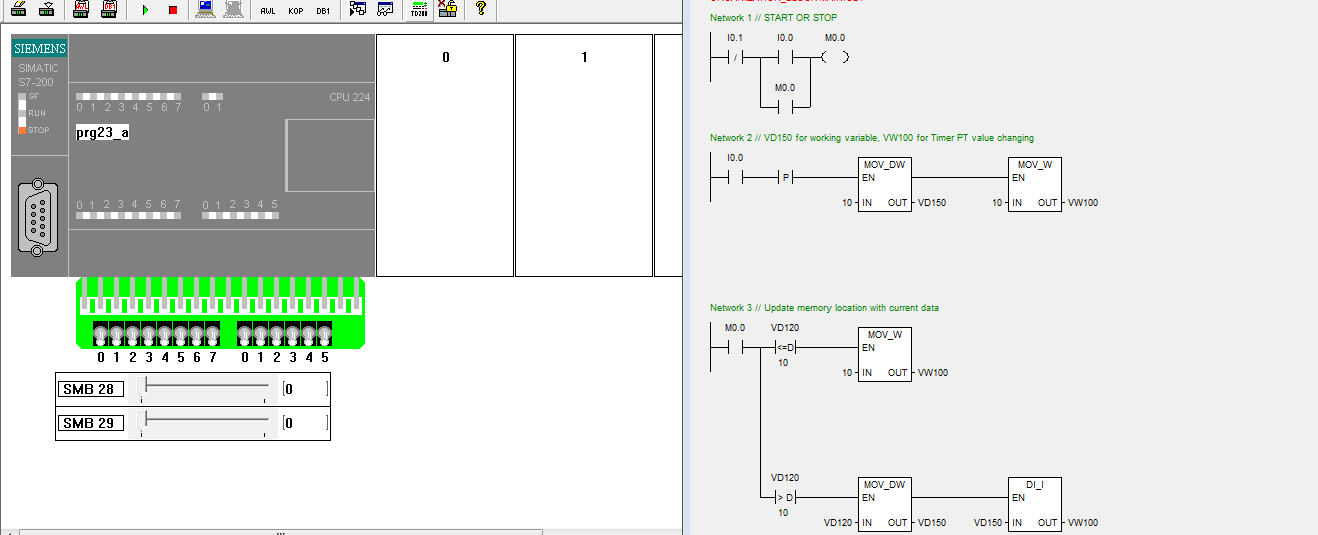
\includegraphics[width = 165mm, scale =0.9]{prg23u1.png}
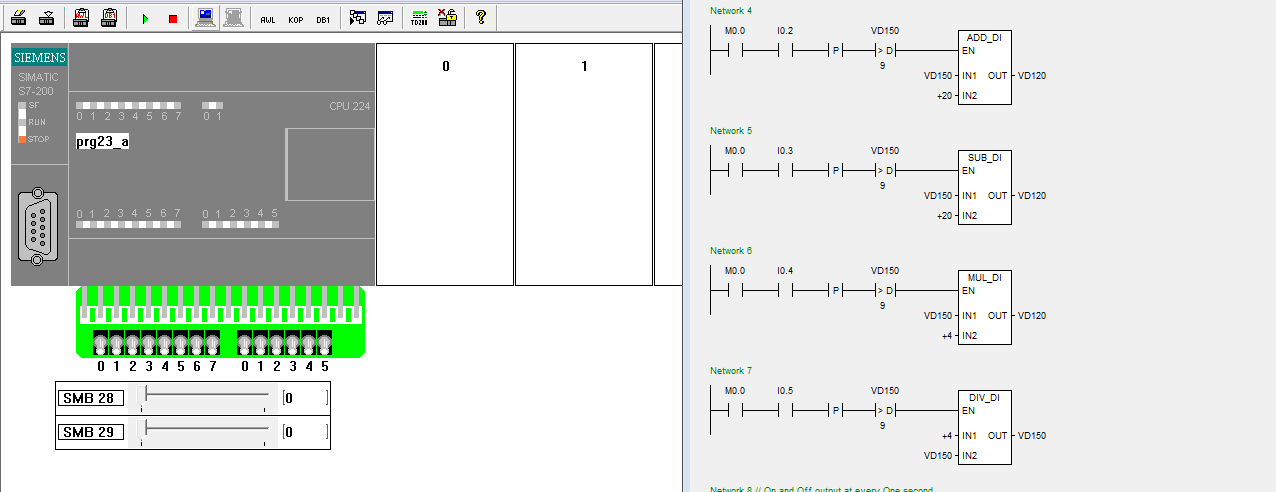
\includegraphics[width = 165mm, scale =0.9]{prg23u2.png}
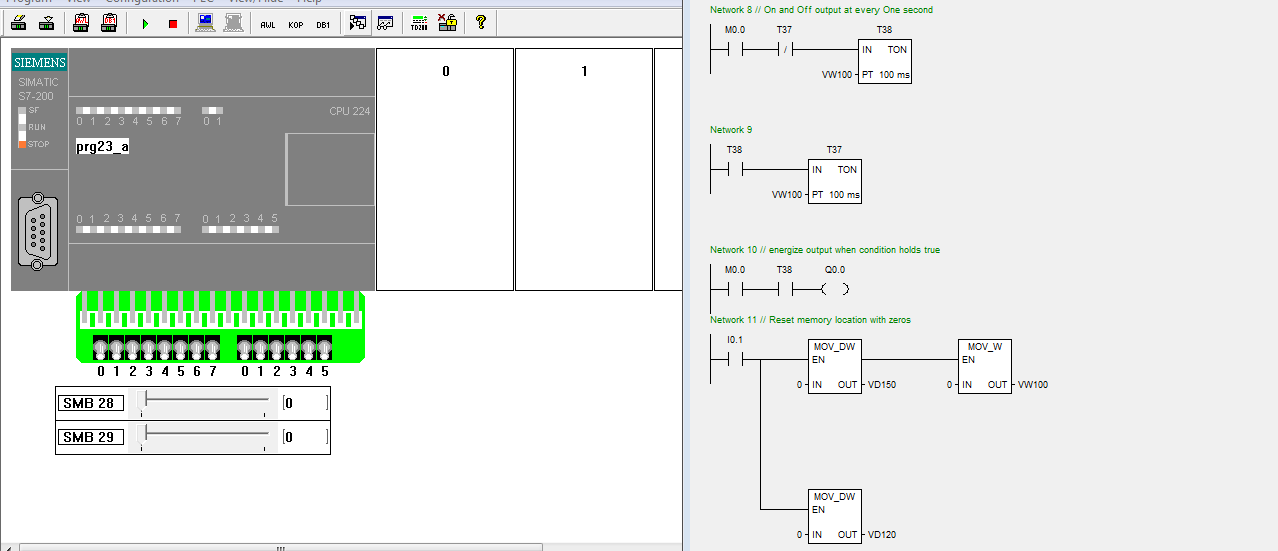
\includegraphics[width = 165mm, scale =0.9]{prg23u3.png}
\end{center}
\section*{Program \#24}
\begin{problem}
 There are three heaters and one RTD sensor with transmitter connected with
 PLC.(eg PLC will read analog value in AIW0 From from 0 to 32000 counts)
 where $0^o C$ to $300^o C$ data transmit by interpolating with current signal of 4 to 20mA  \medskip
 \begin{itemize}
 \item when temp is $\lesssim 60^o$, All three heaters ON
 \item when $60 < temp \lesssim 150$, any Two heaters will be ON
 \item when $150 < temp \lesssim 250$, Only one heater will be ON
 \item when temp > 250 , All heaters should be OFF
 \end{itemize}
\end{problem}

\subsection*{Answer}
 \begin{center}
 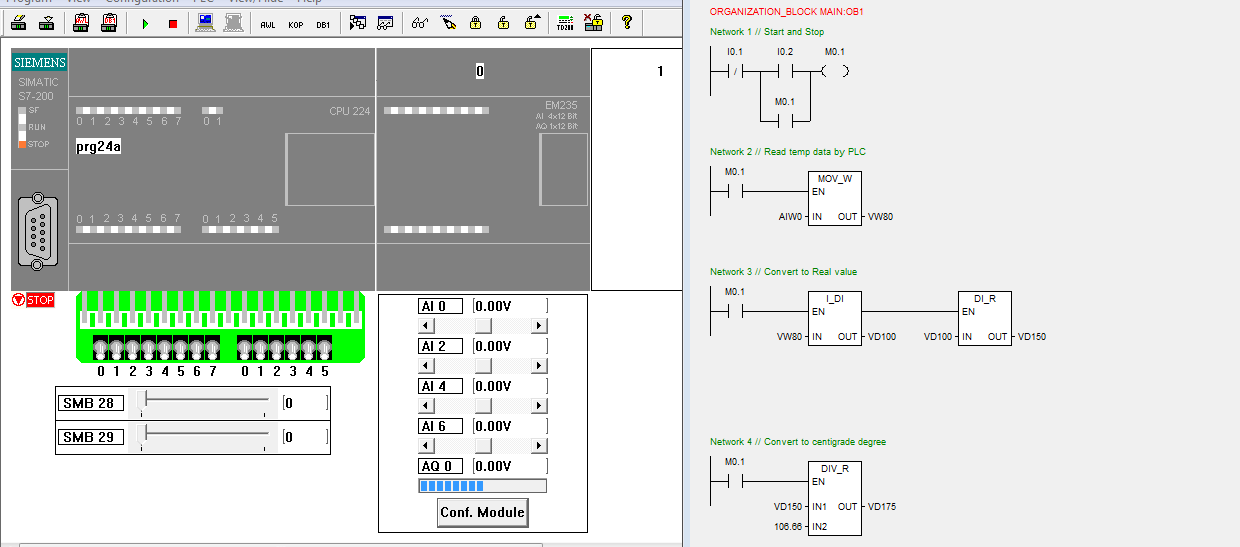
\includegraphics[width = 165mm, scale =0.9]{prg24a.png}
 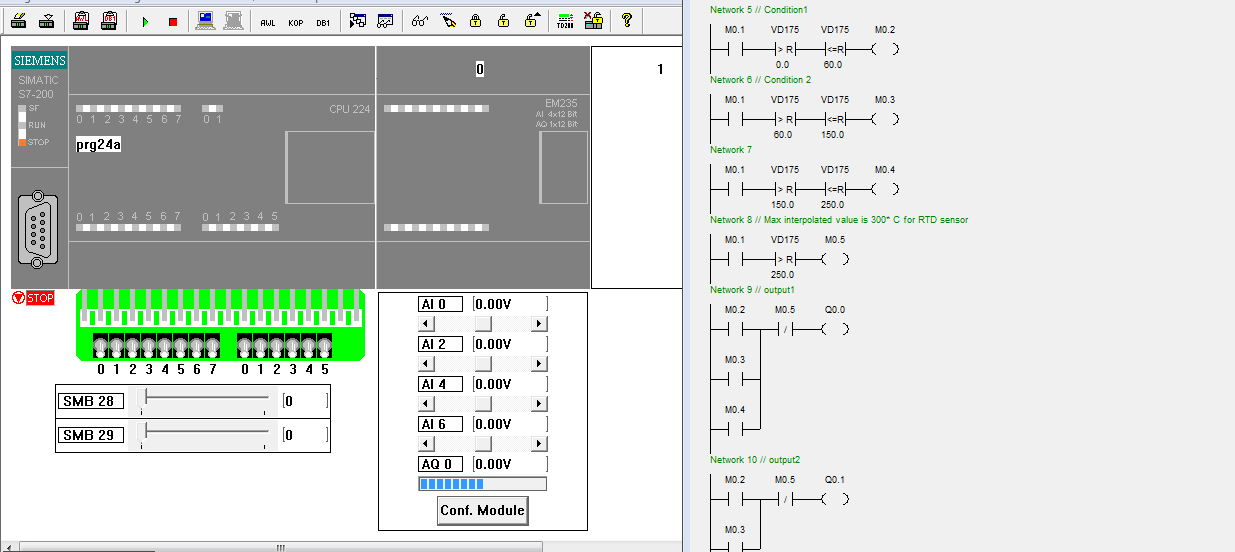
\includegraphics[width = 165mm, scale =0.9]{prg24b.png}
 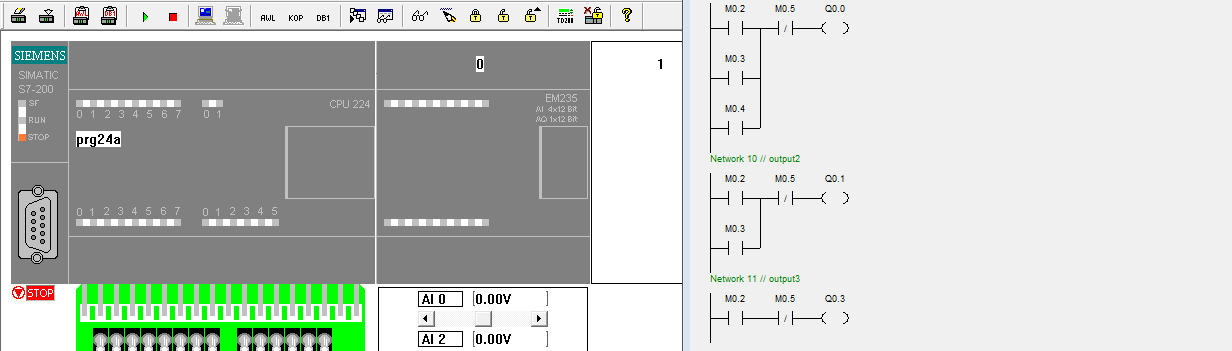
\includegraphics[width = 165mm, scale =0.9]{prg24c.png}
 \end{center}

 \section*{Program \#25}
\begin{problem}
 In a process, there are two sensors and 3 Outputs in which one is pressure
 sensor that is read value from 0 to 6 bar, and one temperature sensor use to
 control three heaters as per below condition. \medskip
 \begin{itemize}
 \item Process is start only if pressure is grater than 3 bar
 \item when temp is less than $50^o C$ all heaters will be ON
 \item when $50^0 C < temp \lesssim 80^o C$ two heaeters will be ON
 \item when $80^0 C < temp \lesssim 150^o C$ only one heater will be ON
 \item when temp > $120^0 C$ All heaters should be OFF
 \end{itemize}
\end{problem}
\subsection*{Answer}
  \begin{center}
  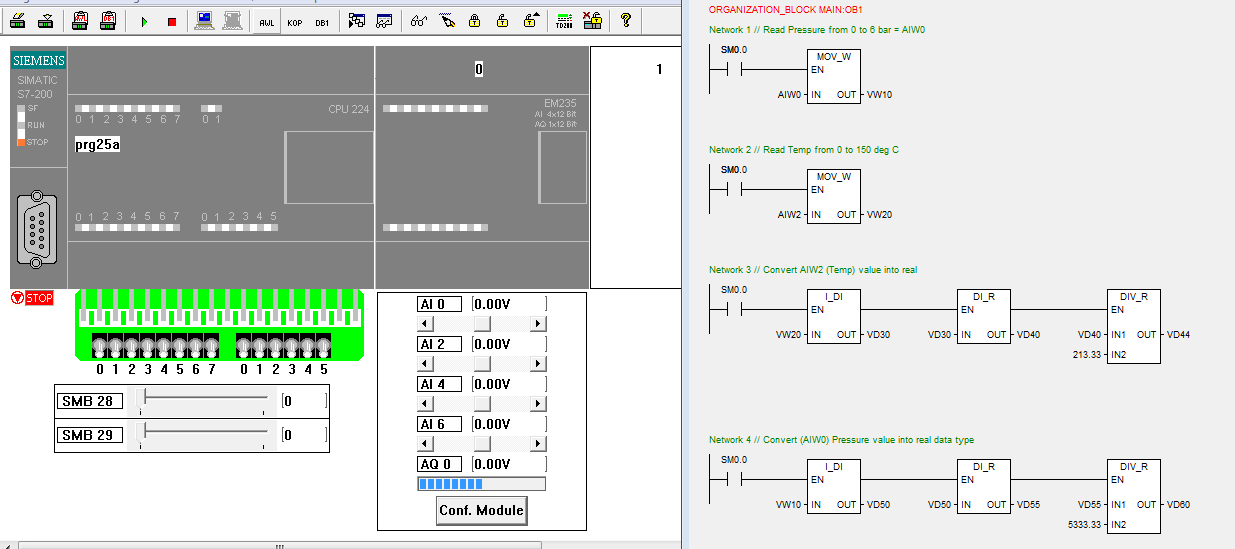
\includegraphics[width = 165mm, scale =0.9]{prg25a.png}
  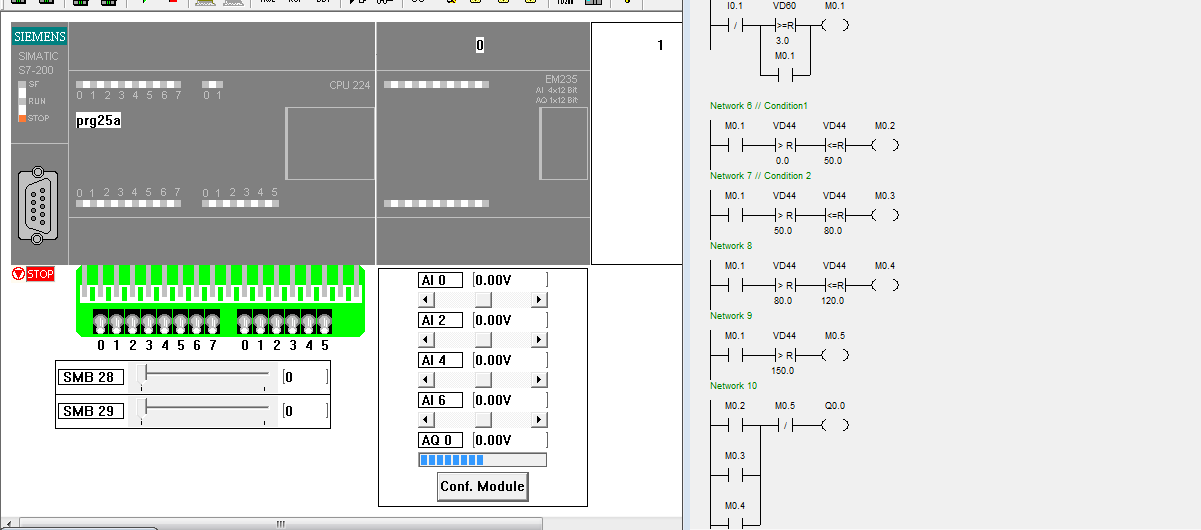
\includegraphics[width = 165mm, scale =0.9]{prg25b.png}
  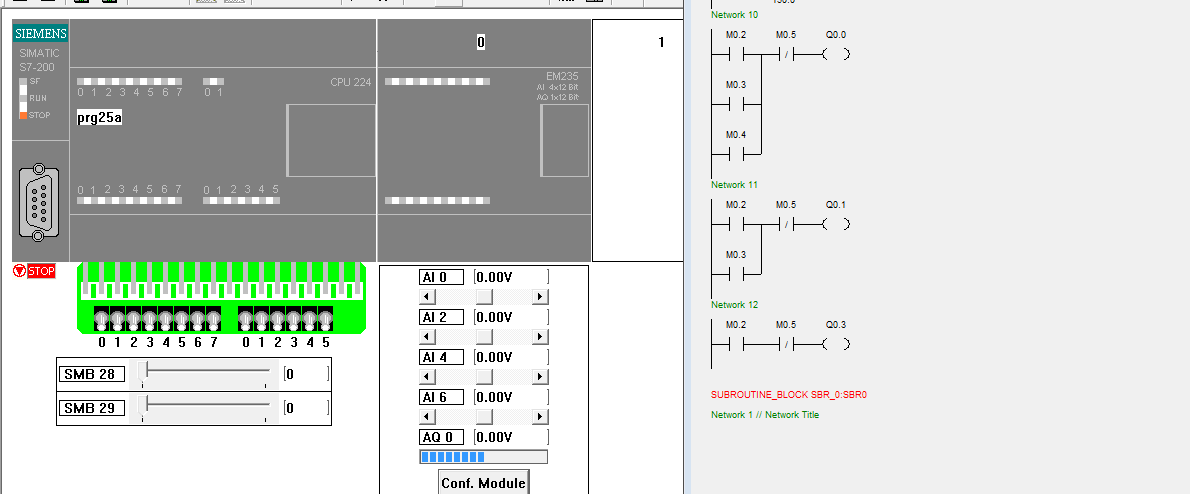
\includegraphics[width = 165mm, scale =0.9]{prg25c.png}
  \end{center}
\section*{Program \#26}
\begin{problem}
  \begin{center}
    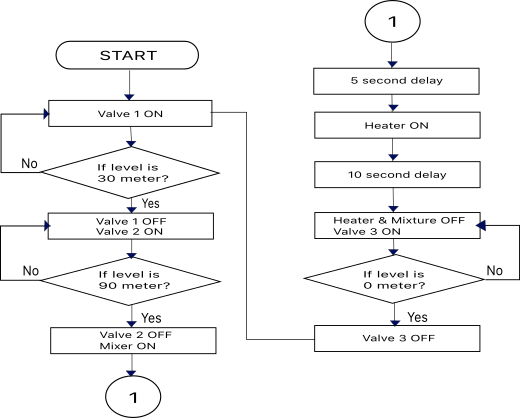
\includegraphics[width = 100mm, scale = 0.9]{heat_mix_1.png}
  \end{center}
  \end{problem}
 \subsection*{Answer}
   \begin{center}
   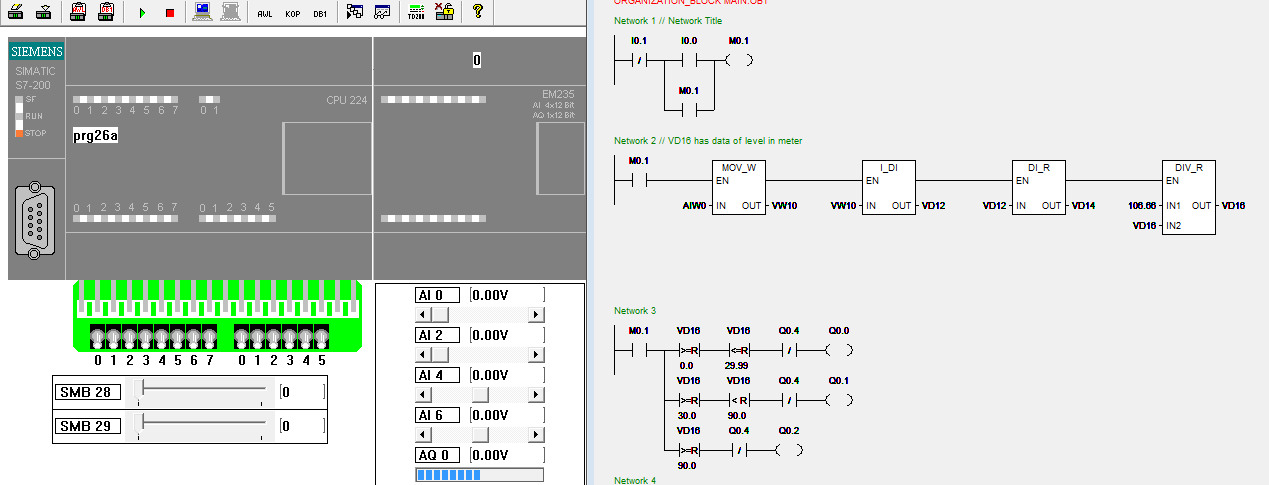
\includegraphics[width = 165mm, scale =0.9]{prg26a1.png}
   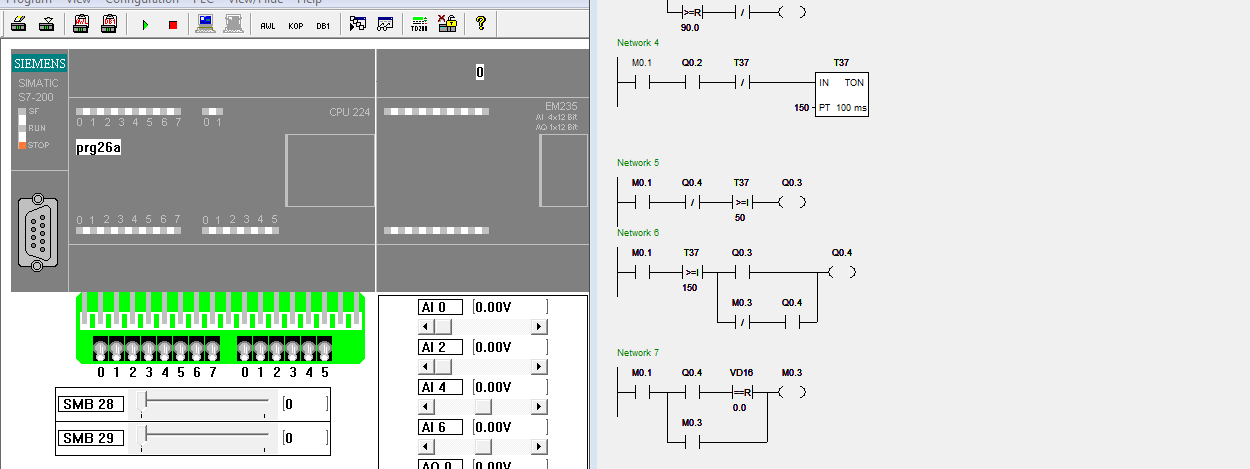
\includegraphics[width = 165mm, scale =0.9]{prg26a2.png}
   \end{center}
    
  \section*{Program \#27}
  \begin{problem}
  \begin{center}
    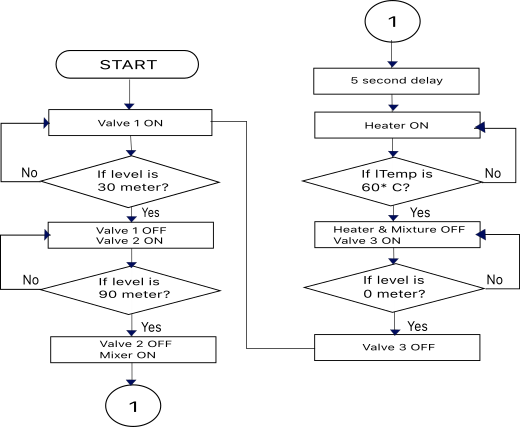
\includegraphics[width = 100mm, scale = 0.9]{heat_mix_2.png}
    \end{center}                                                   
  \end{problem}
  \subsection*{Answer}
    \begin{center}
    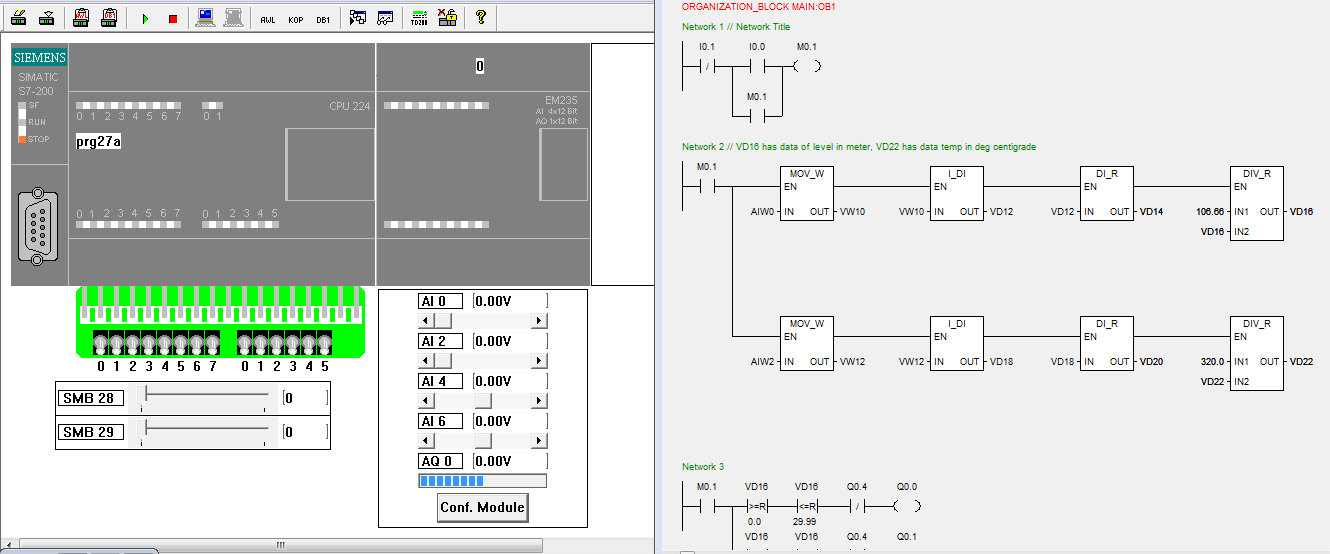
\includegraphics[width = 165mm, scale =0.9]{prg27a1.png}
    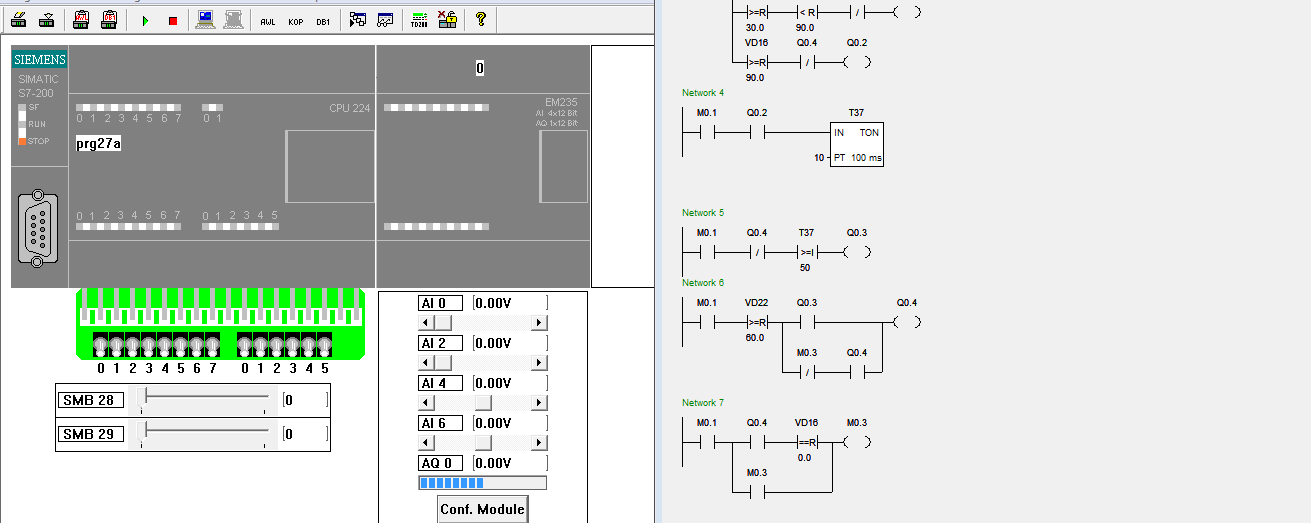
\includegraphics[width = 165mm, scale =0.9]{prg27a2.png}
    \end{center}
  
  \section*{Program \#28}
  \begin{problem}There is one Induction motor with synchronous speed of 1500
    RPM, so design a ladder logic in such a way that IM will start by increasing
    its peed in some
    discrete interval
    as shown in figure. where total time delay to achieve full load speed is 50
    sec given.
\begin{enumerate}
\item Increase speed in 5 such different discrete interval as shown in
  figure
  \begin{center}
    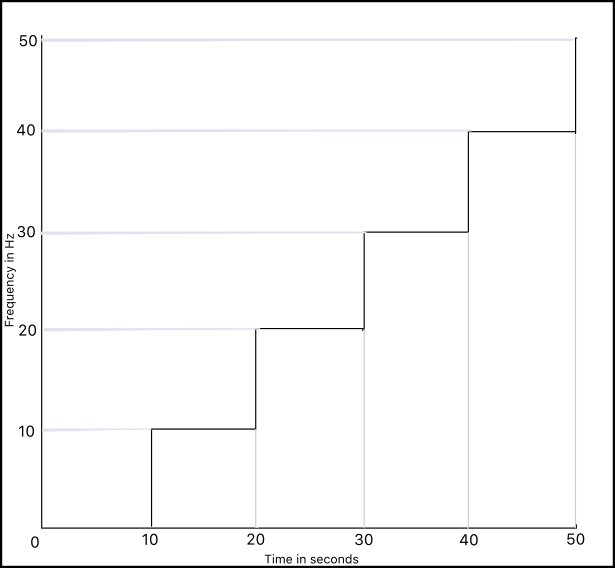
\includegraphics[width = 100mm,height=45mm, scale = 0.8]{draw_28_a.png}
  \end{center}
\item design part(a) with different universal logic
\item increase speed in 50 such different discrete interval, or more
  fine linear increasing manner
  \begin{center}
    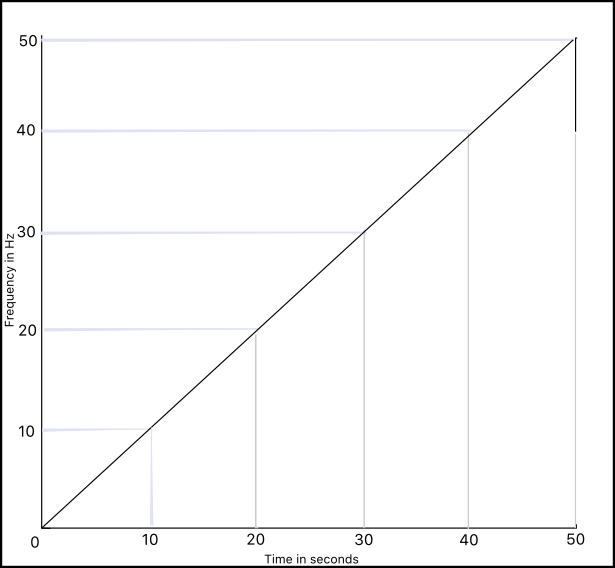
\includegraphics[width = 100mm, height=45mm, scale = 0.8]{draw_28_c.png}
    \end{center}  
\item increase speed with 50 discrete levels in 50 sec and after 100
  sec decrease speed with same levels in same time interval
  \begin{center}
    \includegraphics[width = 100mm, height = 45mm, scale = 0.8]{draw_28_d.png}
    \end{center}                                                
\end{enumerate}
\end{problem}
\pagebreak
\subsection*{Answer}
\begin{enumerate}
\item
  \begin{center}
    \includegraphics[width = 165mm, scale = 0.9]{prg28a1.png}
    \includegraphics[width = 165mm, scale = 0.9]{prg28a2.png}
    \end{center}
\item
    \begin{center}
      \includegraphics[width = 165mm, scale = 0.9]{prg28b1.png}
      \includegraphics[width = 165mm, scale = 0.9]{prg28b2.png}
    \end{center}
  \item
    \begin{center}
      \includegraphics[width = 165mm, scale = 0.9]{prg28c1.png}
      \includegraphics[width = 165mm, scale = 0.9]{prg28c2.png}
    \end{center}
  \item
    \begin{center}
      \includegraphics[width = 165mm, scale = 0.9]{prg28d1.png}
      \includegraphics[width = 165mm, scale = 0.9]{prg28d2.png}
      \includegraphics[width = 165mm, scale = 0.9]{prg28d3.png}
    \end{center}
\end{enumerate}
\end{document}